\subsection{Test case generation}

\subsubsection{Introduction}

\definition{Testing Workflow} is a \textbf{type of software testing that verifies that each software workflow accurately reflects the given business process}. A workflow is a series of tasks to produce a desired result, usually involving several stages or steps. For any business process, testing these sequential steps is defined as \dquotes{workflow testing}.

\begin{figure}[!htp]
    \centering
    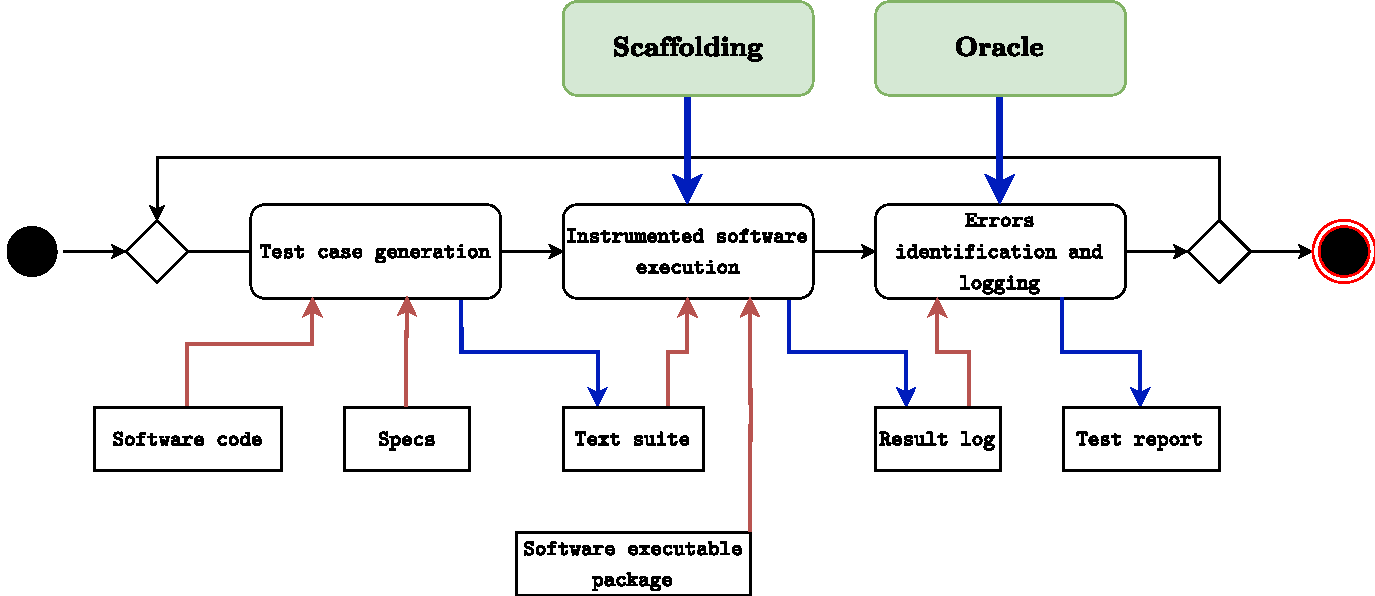
\includegraphics[width=\textwidth]{img/testing-overflow.pdf}
    \caption{Testing Workflow.}
    \label{fig: Testing Workflow}
\end{figure}

\noindent
To view the component diagram in high resolution, scan (or click) the QR code below.
\begin{center}
    \qrcode{https://github.com/PoliMI-HPC-E-notes-projects-AndreVale69/HPC-E-PoliMI-university-notes/tree/main/software-engineering-for-hpc/notes/img/testing-overflow.pdf}
\end{center}

\noindent
As we can see in Figure \ref{fig: Testing Workflow}, test cases can be generated in a \textbf{black-box} or \textbf{white-box} manner. The \definition{White Box} is a \textbf{generation based on code features}. Meanwhile, the \definition{Black Box} is a generation \textbf{based on specification features}.

Test case generation can be done manually (no need to explain) or automatically. Automatic generation can be done in several ways:
\begin{itemize}
    \item \definition{Combinatorial} testing. It enumerates all possible inputs according to some policy (e.g. smaller to larger).
    
    \item \definition{Concolic Execution} (analyzed in the section \ref{subsubsection: Concolic Execution} on page \pageref{subsubsection: Concolic Execution}). It's a pseudo-random generation of inputs guided by symbolic path properties.
    
    \item \definition{Fuzz} testing (\emph{fuzzing}). It's a pseudo-random generation of inputs, including invalid, unexpected inputs.
    
    \item \definition{Search-based} testing. It explores the space of valid inputs, looking for those that improve some metric (e.g. coverage, diversity, fault inducing capability).
    
    \item \definition{Metamorphic} testing. Generates new test cases based on some metamorphic relationships and other previously defined test cases.
\end{itemize}

\newpage

\subsubsection{Concolic Execution}\label{subsubsection: Concolic Execution}

\definition{Concolic Execution} (concrete-symbolic execution) is an \textbf{automatic generation of test cases}. It's a pseudo-random generation of inputs guided by symbolic path properties.

\highspace
In other words, the concolic execution \textbf{performs symbolic execution} (definition on page \pageref{def: symbolic execution}) \textbf{alongside} concrete execution (\textbf{concrete inputs}). Under the hood, in concolic execution a \textbf{state} combines a symbolic part and a concrete part, used as needed to make progress in the exploration.

\highspace
The steps are then as follows:
\begin{itemize}
    \item Concrete $\xrightarrow{\text{to}}$ Symbolic, derive conditions to explore new paths.
    
    \item Symbolic $\xrightarrow{\text{to}}$ Concrete, simplifying conditions to generate concrete inputs.
\end{itemize}
Let's take an example to clarify the explanation.

\begin{examplebox}
    See the code below:
    \lstinputlisting[language=python]{code/concolic-execution-1.py}
    Let's explore all the paths of the \texttt{m2} method, starting with \textbf{a (random) concrete input} and at the \emph{same time} building the \textbf{symbolic condition of the explored path}. Unfortunately, in some cases we will not be able to solve the symbolic execution. For example, the behavior of the first if-condition (\texttt{z == x}) is unknown in the code. For this reason, we execute it with the identified input cases: given \texttt{y = 7}, run \texttt{bb(7)} and return \texttt{14}. With this arrangement, the condition can be solved.

    The annotation used will be the same as in the Symbolic Execution example on page \pageref{example: Symbolic Execution}.

    \begin{enumerate}
        \item Let's start with defined parameters and no condition state:
        \begin{center}
            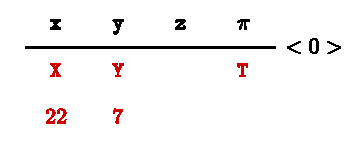
\includegraphics[width=.5\textwidth]{img/concolic-execution-1.pdf}
        \end{center}

        \newpage

        \item Call the function with the parameter \texttt{y}, i.e. value \texttt{7}. The return value of the called function will be \texttt{14}.
        \begin{center}
            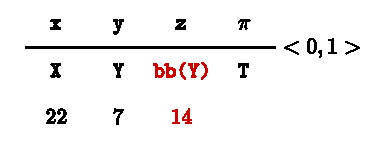
\includegraphics[width=.5\textwidth]{img/concolic-execution-2.pdf}
        \end{center}

        \item The if condition \texttt{14 == 22} is obviously false, so the path will be \texttt{6} and \texttt{7}. By the way, the condition can also be seen as a logical condition $\lnot \left(\texttt{bb}\left(\texttt{Y}\right) \ne \texttt{X}\right)$. But it can't be solved, so the concolic execution goes from symbolic to concrete $\lnot \left(14 \ne \texttt{X}\right) \equiv \texttt{14} = \texttt{X}$.
        \begin{center}
            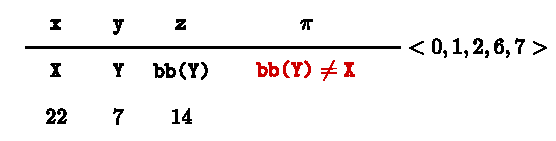
\includegraphics[width=.7\textwidth]{img/concolic-execution-3.pdf}
        \end{center}
    \end{enumerate}

    \longline

    \begin{enumerate}
        \setcounter{enumi}{3}
        \item After a random concrete input, we can solve the constraint and start a new exploration. The parameter value of \texttt{X} is now \texttt{14}. This is because we do not want the condition from the previous step to be \emph{not equal}.
        \begin{center}
            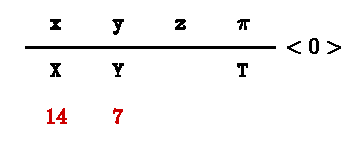
\includegraphics[width=.5\textwidth]{img/concolic-execution-4.pdf}
        \end{center}

        \item The result of the function \texttt{bb(7)} is \texttt{14}.
        \begin{center}
            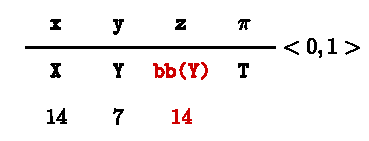
\includegraphics[width=.5\textwidth]{img/concolic-execution-5.pdf}
        \end{center}

        \item Unlike before, the \texttt{if} condition is now true!
        \begin{center}
            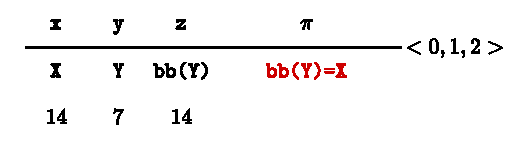
\includegraphics[width=.6\textwidth]{img/concolic-execution-6.pdf}
        \end{center}

        \item The evaluation of the third line of code needs no explanation.
        \begin{center}
            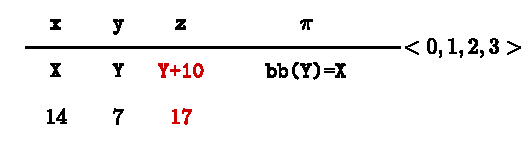
\includegraphics[width=.7\textwidth]{img/concolic-execution-7.pdf}
        \end{center}

        \item The path just explored explores the whole code. To try another path, we can negate the condition, but be careful! We only need to negate the second condition, because we already negated the first condition in the first exploration.
        \begin{equation*}
            \texttt{bb}\left(\texttt{Y}\right) = \texttt{X} \land \texttt{X} \le \texttt{Y+10} \: \Longrightarrow \: \texttt{bb}\left(\texttt{Y}\right) = \texttt{X} \land \texttt{X} > \texttt{Y+10}
        \end{equation*}
        \begin{center}
            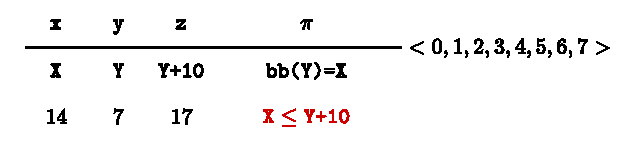
\includegraphics[width=.8\textwidth]{img/concolic-execution-8.pdf}
        \end{center}
    \end{enumerate}

    \longline

    \begin{enumerate}
        \setcounter{enumi}{8}
        \item Explore the new path using two (random) values that satisfy the previous logical condition.
        \begin{center}
            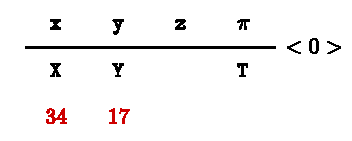
\includegraphics[width=.5\textwidth]{img/concolic-execution-9.pdf}
        \end{center}

        \item The result of the \texttt{bb} function is \texttt{34}.
        \begin{center}
            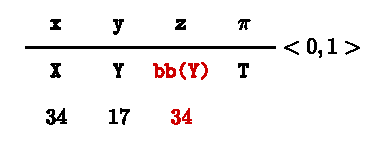
\includegraphics[width=.5\textwidth]{img/concolic-execution-10.pdf}
        \end{center}

        \item The \texttt{if} condition is obviously true.
        \begin{center}
            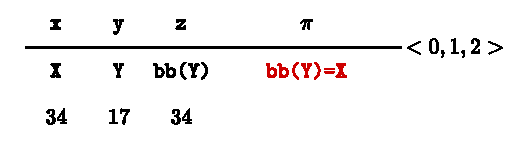
\includegraphics[width=.7\textwidth]{img/concolic-execution-11.pdf}
        \end{center}

        \newpage

        \item We add \texttt{10} to the variable \texttt{Y}.
        \begin{center}
            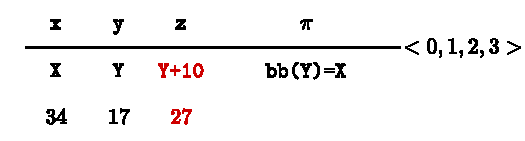
\includegraphics[width=.7\textwidth]{img/concolic-execution-12.pdf}
        \end{center}

        \item In this case the \texttt{if} condition is false and we complete the exercise because we have explored every possible path!
        \begin{center}
            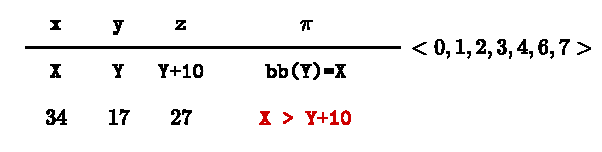
\includegraphics[width=.8\textwidth]{img/concolic-execution-13.pdf}
        \end{center}
    \end{enumerate}
\end{examplebox}

\begin{flushleft}
    \textcolor{Green3}{\faIcon{check} \textbf{Advantages}}
\end{flushleft}
The concolic execution has two main advantages:
\begin{enumerate}
    \item Can \textbf{handle black-box functions in path conditions} (not possible with symbolic execution!).
    \item Can \textbf{automatically generate concrete test cases according to a code coverage criterion}.
\end{enumerate}

\begin{flushleft}
    \textcolor{Red2}{\faIcon{exclamation-triangle} \textbf{Limitations}}
\end{flushleft}
And the disadvantages are:
\begin{enumerate}
    \item It will only \textbf{find one input example per path}. And this could be a problem, because typically the errors only occur with certain inputs. What's more, if the errors are infrequent events, it's difficult to detect them with concolic execution.
    
    \item The number of paths explodes due to complex nested conditions, then it \textbf{requires a large search space}.

    \item It \textbf{doesn't guide the exploration}, it just explores possible paths one by one, as long as we have the budget (e.g. time, number of runs).
\end{enumerate}

\newpage

\subsubsection{Concurrent systems testing}

There are many difficulties in testing concurrent software. For example, the \textbf{concurrency bugs are non-deterministic} and can only manifest themselves within certain \emph{interleavings}. Furthermore, the interleavings depend on execution conditions that are not under the direct control of the program.

\begin{examplebox}
    The following code:
    \lstinputlisting{code/different-interleavings}
    Can have the following possible execution behaviors:
    \begin{center}
        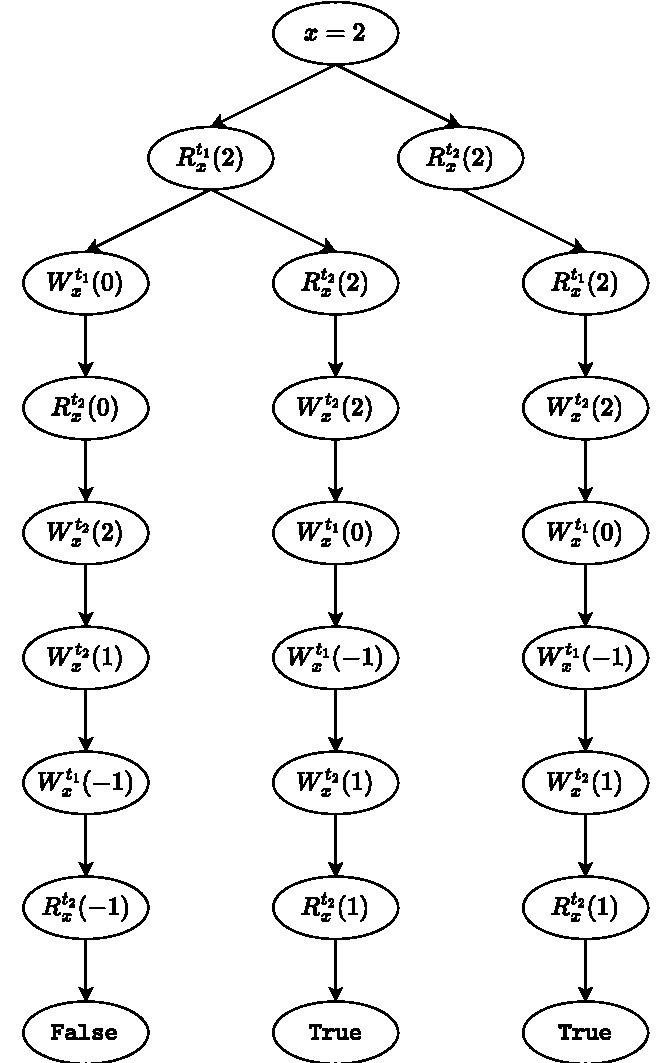
\includegraphics[width=.6\textwidth]{img/different-interleavings-2.pdf}
    \end{center}
\end{examplebox}

\newpage

\begin{examplebox}[: an example of data race]
    \lstinputlisting{code/data-race}
\end{examplebox}

\begin{examplebox}[: an example of atomicity violation]
    \lstinputlisting{code/atomicity-violation}
\end{examplebox}

\begin{examplebox}[: an example of deadlock]
    \lstinputlisting{code/deadlock}
\end{examplebox}

\begin{flushleft}
    \textcolor{Green3}{\faIcon{question-circle} \textbf{So how do you test concurrent programmes?}}
\end{flushleft}
\definition{Metamorphic Testing (MT)} is a property-based software testing technique that can be an effective approach to solving the test oracle problem\footnote{In software testing, a \textbf{Test Oracle} (or simply oracle) is a provider of information that describes the correct output based on the input of a test case.} and the test case generation problem (this chapter). The test oracle problem is the difficulty in determining the expected results of selected test cases, or whether the actual results match the expected results.

\highspace
The MT technique is applicable to any type of software and has recently been \textbf{adapted to detect \emph{data race} problems} in concurrent software.

\highspace
The basic idea of general MT is to derive \definition{Metamorphic Relations (MRs)} between multiple program inputs and corresponding outputs:
\begin{enumerate}
    \item New test cases from existing ones
    \item An oracle for the program
\end{enumerate}

\begin{examplebox}
    Consider a program $P$ computing the shortest path in an undirected graph $G$. We may express the following properties (MRs):
    \begin{enumerate}[label=\textbf{MR\arabic*}]
        \item The length of the shortest path between two points in the graph doesn't vary if we swap the two points:
        \begin{equation*}
            \left| P\left(G,a,b\right) \right| = \left| P\left(G,b,a\right) \right|
        \end{equation*}

        \item If $c$ belongs to the shortest path between $a$ and $b$:
        \begin{equation*}
            \left| P\left(G,a,c\right) \right| + \left| P\left(G,c,b\right) \right| = \left| P\left(G,a,b\right) \right|
        \end{equation*}
    \end{enumerate}
    Now we can:
    \begin{enumerate}
        \item Pick a source test case $<a1, b1>$ selected with any technique;
        \item Run the software and obtain the result, that is, the shortest path and its length
        \item Based on MR1, generate a follow up test case $<b1, a1>$
        \item Run the software with the new test case
        \item Check if MR holds: 
        \begin{equation*}
            \left| P\left(G,a1,b1\right) \right| = \left| P\left(G,b1,a1\right) \right|
        \end{equation*}
        If not, then $P$ is failing.
    \end{enumerate}
\end{examplebox}